%%%%%%%%%%%%%%%%%%%%%%%%%%%%%%%%%%%%%%%%%%%%%%%%%%%%%%%%%%%%%%%%%%%%%%
%%  disstemplate.tex, to be compiled with latex.             %
%%  08 April 2002   Version 4                    %
%%%%%%%%%%%%%%%%%%%%%%%%%%%%%%%%%%%%%%%%%%%%%%%%%%%%%%%%%%%%%%%%%%%%%%
%%                                   %
%%  Writing a Doctoral Dissertation with LaTeX at            %
%%  the University of Texas at Austin                %
%%                                   %
%%  (Modify this ``template'' for your own dissertation.)        %
%%                                   %
%%%%%%%%%%%%%%%%%%%%%%%%%%%%%%%%%%%%%%%%%%%%%%%%%%%%%%%%%%%%%%%%%%%%%%


\documentclass[12pt]{report}    % The documentclass must be ``report''.

\usepackage{utdiss2}        % Dissertation package style file.


%%%%%%%%%%%%%%%%%%%%%%%%%%%%%%%%%%%%%%%%%%%%%%%%%%%%%%%%%%%%%%%%%%%%%%
% Optional packages used for this sample dissertation. If you don't  %
% need a capability in your dissertation, feel free to comment out   %
% the package usage command.                         %
%%%%%%%%%%%%%%%%%%%%%%%%%%%%%%%%%%%%%%%%%%%%%%%%%%%%%%%%%%%%%%%%%%%%%%

\usepackage{amsmath,amsthm,amsfonts,amscd}
                % Some packages to write mathematics.
\usepackage{eucal}      % Euler fonts
\usepackage{fancyvrb}                                       % For code environment
\DefineVerbatimEnvironment{code}{Verbatim}{fontsize=\small} %
\usepackage{makeidx}        % Package to make an index.
\usepackage{psfig}          % Allows inclusion of eps files.
\usepackage{epsfig}             % Allows inclusion of eps files.
\usepackage{citesort}           %
\usepackage{url}        % Allows good typesetting of web URLs.
%\usepackage{draftcopy}     % Uncomment this line to have the
                % word, "DRAFT," as a background
                % "watermark" on all of the pages of
                % of your draft versions. When ready
                % to generate your final copy, re-comment
                % it out with a percent sign to remove
                % the word draft before you re-run
                % Makediss for the last time.



\author{Edward Amsden }    % Required

\address{13567 McCartyville Road \\ Anna, Ohio 45302}  % Required

\title{TimeFlies: \\ Push-Pull Signal-Function \\ Functional Reactive Programming}
                                                    % Required

%%%%%%%%%%%%%%%%%%%%%%%%%%%%%%%%%%%%%%%%%%%%%%%%%%%%%%%%%%%%%%%%%%%%%%
% NOTICE: The total number of supervisors and other members %%%%%%%%%%
%%%%%%%%%%%%%%% MUST be seven (7) or less! If you put in more, %%%%%%%
%%%%%%%%%%%%%%% they are put on the page after the Committee %%%%%%%%%
%%%%%%%%%%%%%%% Certification of Approved Version page. %%%%%%%%%%%%%%
%%%%%%%%%%%%%%%%%%%%%%%%%%%%%%%%%%%%%%%%%%%%%%%%%%%%%%%%%%%%%%%%%%%%%%

%%%%%%%%%%%%%%%%%%%%%%%%%%%%%%%%%%%%%%%%%%%%%%%%%%%%%%%%%%%%%%%%%%%%%%
%
% Enter names of the supervisor and co-supervisor(s), if any,
% of your dissertation committee. Put one name per line with
% the name in square brackets. The name on the last line, however,
% must be in curly braces.
%
% If you have only one supervisor, the entry below will read:
%
%   \supervisor
%       {Supervisor's Name}
%
% NOTE: Maximum three supervisors. Minimum one supervisor.
% NOTE: The Office of Graduate Studies will accept only two supervisors!
%
%
\supervisor
    {Dr. Matthew Fluet}

%%%%%%%%%%%%%%%%%%%%%%%%%%%%%%%%%%%%%%%%%%%%%%%%%%%%%%%%%%%%%%%%%%%%%%
%
% Enter names of the other (non-supervisor) members(s) of your
% dissertation committee. Put one name per line with the name
% in square brackets. The name on the last line, however, must
% be in curly braces.
%
% NOTE: Maximum six other members. Minimum zero other members.
% NOTE: The Office of Graduate Studies may restrict you to a total
%   of six committee members.
%
%
\committeemembers
%    [Erwin Schr\"odinger]
    [Arthur Nunes-Harwitt, Reader]
    {Dr. Zach Butler, Observer}
%    {Arthur Schawlow}

%%%%%%%%%%%%%%%%%%%%%%%%%%%%%%%%%%%%%%%%%%%%%%%%%%%%%%%%%%%%%%%%%%%%%%

\previousdegrees{B.S.}
     % The abbreviated form of your previous degree(s).
     % E.g., \previousdegrees{B.S., MBA}.
     %
     % The default value is `B.S., M.S.'

\graduationmonth{August}
     % Graduation month, either May, August, or December, in the form
     % as `\graduationmonth{May}'. Do not abbreviate.
     %
     % The default value (either May, August, or December) is guessed
     % according to the time of running LaTeX.

\graduationyear{2013}
     % Graduation year, in the form as `\graduationyear{2001}'.
     % Use a 4 digit (not a 2 digit) number.
     %
     % The default value is guessed according to the time of
     % running LaTeX.

%\typist{...}
     % The name(s) of typist(s), put `the author' if you do it yourself.
     % E.g., `\typist{Maryann Hersey and the author}'.
     %
     % The default value is `the author'.


%%%%%%%%%%%%%%%%%%%%%%%%%%%%%%%%%%%%%%%%%%%%%%%%%%%%%%%%%%%%%%%%%%%%%%
% Commands for master's theses and reports.              %
%%%%%%%%%%%%%%%%%%%%%%%%%%%%%%%%%%%%%%%%%%%%%%%%%%%%%%%%%%%%%%%%%%%%%%
%
% If the degree you're seeking is NOT Doctor of Philosophy, uncomment
% (remove the % in front of) the following two command lines (the ones
% that have the \ as their second character).
%
\degree{Master of Science} \degreeabbr{M.S.}

% Uncomment the line below that corresponds to the type of master's
% document you are writing.
%
%\masterreport
\masterthesis


%%%%%%%%%%%%%%%%%%%%%%%%%%%%%%%%%%%%%%%%%%%%%%%%%%%%%%%%%%%%%%%%%%%%%%
% Some optional commands to change the document's defaults.      %
%%%%%%%%%%%%%%%%%%%%%%%%%%%%%%%%%%%%%%%%%%%%%%%%%%%%%%%%%%%%%%%%%%%%%%
%
%\singlespacing
%\oneandonehalfspacing

%\singlespacequote
\oneandonehalfspacequote

\topmargin 0.125in  % Adjust this value if the PostScript file output
            % of your dissertation has incorrect top and
            % bottom margins. Print a copy of at least one
            % full page of your dissertation (not the first
            % page of a chapter) and measure the top and
            % bottom margins with a ruler. You must have
            % a top margin of 1.5" and a bottom margin of
            % at least 1.25". The page numbers must be at
            % least 1.00" from the bottom of the page.
            % If the margins are not correct, adjust this
            % value accordingly and re-compile and print again.
            %
            % The default value is 0.125"

        % If you want to adjust other margins, they are in the
        % utdiss2-nn.sty file near the top. If you are using
        % the shell script Makediss on a Unix/Linux system, make
        % your changes in the utdiss2-nn.sty file instead of
        % utdiss2.sty because Makediss will overwrite any changes
        % made to utdiss2.sty.

%%%%%%%%%%%%%%%%%%%%%%%%%%%%%%%%%%%%%%%%%%%%%%%%%%%%%%%%%%%%%%%%%%%%%%
% Some optional commands to be tested.                   %
%%%%%%%%%%%%%%%%%%%%%%%%%%%%%%%%%%%%%%%%%%%%%%%%%%%%%%%%%%%%%%%%%%%%%%

% If there are 10 or more sections, 10 or more subsections for a section,
% etc., you need to make an adjustment to the Table of Contents with the
% command \longtocentry.
%
%\longtocentry



%%%%%%%%%%%%%%%%%%%%%%%%%%%%%%%%%%%%%%%%%%%%%%%%%%%%%%%%%%%%%%%%%%%%%%
%   Some math support.                       %
%%%%%%%%%%%%%%%%%%%%%%%%%%%%%%%%%%%%%%%%%%%%%%%%%%%%%%%%%%%%%%%%%%%%%%
%
%   Theorem environments (these need the amsthm package)
%
%% \theoremstyle{plain} %% This is the default

\newtheorem{thm}{Theorem}[section]
\newtheorem{cor}[thm]{Corollary}
\newtheorem{lem}[thm]{Lemma}
\newtheorem{prop}[thm]{Proposition}
\newtheorem{ax}{Axiom}

\theoremstyle{definition}
\newtheorem{defn}{Definition}[section]

\theoremstyle{remark}
\newtheorem{rem}{Remark}[section]
\newtheorem*{notation}{Notation}

%\numberwithin{equation}{section}


%%%%%%%%%%%%%%%%%%%%%%%%%%%%%%%%%%%%%%%%%%%%%%%%%%%%%%%%%%%%%%%%%%%%%%
%   Macros.                              %
%%%%%%%%%%%%%%%%%%%%%%%%%%%%%%%%%%%%%%%%%%%%%%%%%%%%%%%%%%%%%%%%%%%%%%
%
%   Here some macros that are needed in this document:


\newcommand{\latexe}{{\LaTeX\kern.125em2%
                      \lower.5ex\hbox{$\varepsilon$}}}

\newcommand{\amslatex}{\AmS-\LaTeX{}}

\chardef\bslash=`\\ % \bslash makes a backslash (in tt fonts)
            %   p. 424, TeXbook

\newcommand{\cn}[1]{\texttt{\bslash #1}}

\makeatletter       % Starts section where @ is considered a letter
            % and thus may be used in commands.
\def\square{\RIfM@\bgroup\else$\bgroup\aftergroup$\fi
  \vcenter{\hrule\hbox{\vrule\@height.6em\kern.6em\vrule}%
                                              \hrule}\egroup}
\makeatother        % Ends sections where @ is considered a letter.
            % Now @ cannot be used in commands.

\makeindex    % Make the index

%%%%%%%%%%%%%%%%%%%%%%%%%%%%%%%%%%%%%%%%%%%%%%%%%%%%%%%%%%%%%%%%%%%%%%
%       The document starts here.                %
%%%%%%%%%%%%%%%%%%%%%%%%%%%%%%%%%%%%%%%%%%%%%%%%%%%%%%%%%%%%%%%%%%%%%%

\begin{document}

%\copyrightpage          % Produces the copyright page.


%
% NOTE: In a doctoral dissertation, the Committee Certification page
%       (with signatures) is BEFORE the Title page.
%   In a masters thesis or report, the Signature page
%       (with signatures) is AFTER the Title page.
%
%   If you are writing a masters thesis or report, you MUST REVERSE
%   the order of the \commcertpage and \titlepage commands below.
%
\titlepage              % Produces the title page.
\commcertpage           % Produces the Committee Certification
            %   of Approved Version page (doctoral)
            %   or Signature page (masters).
            %       20 Mar 2002 cwm




%%%%%%%%%%%%%%%%%%%%%%%%%%%%%%%%%%%%%%%%%%%%%%%%%%%%%%%%%%%%%%%%%%%%%%
% Dedication and/or epigraph are optional, but must occur here.      %
%%%%%%%%%%%%%%%%%%%%%%%%%%%%%%%%%%%%%%%%%%%%%%%%%%%%%%%%%%%%%%%%%%%%%%
%
%\begin{dedication}
%\index{Dedication@\emph{Dedication}}%
%Dedicated to my wife Shirley.
%\end{dedication}


\begin{acknowledgments}     % Optional
\index{Acknowledgments@\emph{Acknowledgments}}%
I wish to thank the many people who have supported me as I pursued this work. In particular,
my supervisor Dr. Matthew Fluet was both encouraging and challenging as I explored the question posed
by this thesis, and through the long process of revisions and preparing for my defense.
Professor Arthur Nunes-Harwitt's and Dr. Zack Butler's feedback and contributions were invaluable.
I would also like to thank Dr. Ryan Newton for his understanding and encouragement as I worked concurrently
on the beginning of my PhD studies and this thesis. I thank my family, my mother and father in particular, for
their encouragement and support of my education, and for all of the teaching they so diligently gave me to
enable me to reach this point. Finally and most importantly, \textit{Soli Deo gloria}.
\end{acknowledgments}


% The abstract is required. Note the use of ``utabstract'' instead of
% ``abstract''! This was necessary to fix a page numbering problem.
% The abstract heading is generated automatically.
% Do NOT use \begin{abstract} ... \end{abstract}.
%
\utabstract
\index{Abstract}%
\indent
\begin{abstract}
Functional Reactive Programming is a promising \new{approach} 
\rn{systems -- seems weird to identify it with the implementations... model, approach?} 
for writing interactive and time-dependent programs. Signal-function FRP 
is variant of FRP 
% a subclass of these systems 
which provides advantages in modularity and correctness, but
has proven difficult to implement efficiently.

\textred{The abstraction of signal vectors provides the necessary type apparatus to
distinguish components of the input and output of signal functions which benefit
from a push-based implementation from those which benefit from a pull-based
implementation, and to combine both implementation strategies in a single system.}

\rn{Without understanding it a priori, the above para is hard to
  parse.  How about the following?}

\new{One important implementation trade-off is whether evaluation 
% of a composition 
of signal functions is {\em push-based} or {\em pull-based}.
The {\em signal-vector} technique addresses this by providing a type-level
  description of the inputs and outputs of signal functions, 
  distinguishing} components that benefit from a push-based
implementation from those that benefit from a pull-based
implementation.  This makes it possible to combine both implementation
strategies in a single system.

We describe a \new{novel} \rn{is it novel? how? need clear contributions}
 signal-function FRP system which provides push-based evaluation
for events, pull-based evaluation for signals, and a simple monadic evaluation
interface that permits the system to easily integrate with one or more
IO systems.
\end{abstract}




\tableofcontents   % Table of Contents will be automatically
                   % generated and placed here.

%\listoftables     % List of Tables and List of Figures will be placed
\listoffigures     % here, if applicable.



%%%%%%%%%%%%%%%%%%%%%%%%%%%%%%%%%%%%%%%%%%%%%%%%%%%%%%%%%%%%%%%%%%%%%%
% Actual text starts here.                       %
%%%%%%%%%%%%%%%%%%%%%%%%%%%%%%%%%%%%%%%%%%%%%%%%%%%%%%%%%%%%%%%%%%%%%%
%
% Including external files for each chapter makes this document simpler,
% makes each chapter simpler, and allows for generating test documents
% with as few as zero chapters (by commenting out the include statements).
% This allows quicker processing by the Makediss command file in case you
% are not working on a specific, long and slow to compile chapter. You
% can even change the chapter order by merely interchanging the order
% of the include statements (something I found helpful in my own
% dissertation).
%

\chapter{Introduction}
\label{chapter:Introduction}

Most of the useful programs which programmers are asked to write must react to inputs which are not available at the time the program starts,
and produce effects at many different times throughout the execution of the program. Examples of these programs include GUI applications,
web browsers, web applications, video games, multimedia authoring and playback tools, operating system shells and kernels, servers,
robotic control programs, and many others. This attribute of a program is called reactivity.

Functional reactive programming (FRP) is a promising class of abstractions for
writing interactive programs in functional languages. The FRP abstractions are
{\em behaviors} (also termed {\em signals}), which are functions of continuous
time, and {\em events}, which are sequences of time-value pairs. These
abstractions translate desirable properties of the underlying functional
languages, such as higher-order functions and referential transparency, to
reactive constructs, generally without modifications to the underlying language.
This permits the compositional construction of reactive programs in purely
functional languages.

Functional reactive programming was introduced, though not quite by name, with
Fran~\cite{Elliott1997}, a compositional system for writingm reactive
animations. From the start, two key challenges emerged: the enforcement of
{\em causality}\footnote{Causality is the property that a value in an FRP
program depends only on present and past values. Obviously, a program which
violates this property is impossible to evaluate, but in some FRP systems such
programs are unfortunately quite easy to write down.} in FRP programs, and the
efficient evaluation of FRP programs.

The first challenge was addressed by representing FRP programs, not as
compositions of behaviors and events, but as compositions of transformers of
behaviors and events called {\em signal functions}. By not permitting direct
access to behaviors or events, but representing them implicitly, signal
functions prohibit accessing past or future time values, only allowing access to
values in the closure of the signal function and current input values. Signal
function FRP programs are written by composing signal functions, and are
evaluated using a function which provides input to the signal function and acts
on the output values. This evaluation function is generally elided in existing
literature on signal functions, but we provide a documented and improved
interface for evaluating signal functions. A further advantage of
signal-function FRP programs is that they are more readily composed,
since additional signal functions may be composed on the input or output side of
a signal function, rather than simply the output side as in classic
(non-signal-function) FRP systems.

The second challenge was addressed for classic FRP by the creation of a hybrid
push-pull FRP system~\cite{Elliott2009}. This system relied on the distinction
between reactivity and time dependence to decompose behaviors into phases of
constant or simply time-dependent values, with new phases initiated by event
occurrences. However, this implementation did not address concerns of causality
or composability. Further, the existence of events as first-class values in
classic FRP forced the use of an impure and resource-leaking technique to
compare events when merging, in order to determine which event had the first
occurrence after the current time. Further, since the classic FRP interface
permits access to only the output of a behavior or event, and is always bound to
its implicit inputs, the best the push-based implementation can do is to block
when no computation needs to be performed. The computation cannot be suspended
entirely as a value representation.

To address both challenges in a FRP implementation, we combine the approaches
and demonstrate a push-pull signal-function FRP system. The current
implementation approach for signal-function FRP is inherently
pull-based~\cite{Nilsson2002}, but recent work on N-ary
FRP~\cite{Sculthorpe2011}, a variant of signal-function FRP which enumerates
inputs and distinguishes between events and behaviors, provides a representation
which suggests a method of push-based evaluation. In previous implementations of
signal-function FRP, events were simply option-valued behaviors. This approach has
the advantage of being simple to implement. However, it does not have an obvious
semantics for event merging. Further, it necessitates pull-based evaluation,
since there is no way to separate the events which may be pushed from the truly
continuous values which must be repeatedly sampled.

This thesis describes the design and implementation of TimeFlies, a push-pull signal-function FRP system. This system is presented as a library
of combinators for constructing and evaluating FRP programs.

\chapter{Background}
\label{chapter:Background}

The key abstraction of functional programming is the function, which takes an input and produces an output. Functions may produces functions
as output and/or take functions as input. We say that functions are {\em first-class values} in a language.

Most reactive programs are written in an imperative style, using low-level and non-composable abstractions including callbacks
or object-based event handlers, called by event loops. This ties the model of interactivity to low-level implementation details such as timing and event handling models. 

FRP implies that a model should keep the characteristics of functional programming (i.e. that the basic constructs of the language
should remain first-class) while incorporating reactivity into the language model. In particular, functions should be lifted to operate on reactive values,
and functions themselves ought to be reactive.

The goal of FRP is to provide compositional and high-level abstractions for creating reactive programs. The key
abstractions of FRP are behaviors or signals\footnote{Behaviors are generally referred to as {\em signals} in signal function literature. This is unfortunate, since a signal
function may operate on events, signals, or some combination of the two.}, which are time-dependent values defined at every point in continuous time, and events, which are 
values defined at countably many points in time. An FRP system will provide functions to manipulate events and signals and to react
to events by replacing a portion of the running program in response to an event. Behaviors and events, or some abstraction
based on them, will be first class, in keeping with the spirit of functional programming. Programs implemented in functional reactive
models should of course be efficiently executable. This has proven to be the main challenge in implementing Functional Reactive Programming.

The two general approaches to FRP are ``classic'' FRP, where behaviors and signals are first-class and reactive objects, and ``signal-function'' FRP,
where transformers of signals and events are first-class and reactive objects.

\section{Classic FRP}
\label{section:Background-classic_frp}

The first FRP system, Fran~\cite{Elliott1997}, was introduced as a system for compositionally describing interactive animations.
Though the term ``Functional Reactive Programming'' was not used in this work, it was the first to introduce the concept of first-class
behaviors and events as an abstract model for reactive programs. The key motivation was to separate the implementation of reactivity
from the modelling of reactivity, so that a programmer could be freed from details such as sampling time-varying values, time-slicing
to simulate updating values in parallel, and sampling of inputs.

The first implementation of FRP outside the Haskell language was Frapp\'{e}, an FRP implementation for the Java Beans framework. Frapp\'{e} built on
the notion of events and {\em bound properties} in the Beans framework, providing abstract interfaces for FRP events and behaviors, and combinators
as concrete classes implementing these interfaces. The evaluation of Frapp\'{e} used Bean components as sources and sinks, and the implementation of
Bean events and bound properties to propagate changes to the network~\cite{Courtney2001-2}.


The FrTime\footnote{FrTime is available in the current version of Dr Racket (5.2.1).}~\cite{Cooper2006} language extends the Scheme evaluator with a mutable
dependency graph, which is constructed by program evaluation. This graph is then updated by signal changes. FrTime does not provide a distinct concept of
events, and chooses branches of the dependency graph by conditional evaluation of signals, rather than by the substitution of signals used by FRP systems.

The Reactive~\cite{Elliott2009} system is a push-based FRP system with first-class behaviors and events. The primary insight of Reactive is
the separation of reactivity (or changes in response to events whose occurrence time could not be know beforehand) from time-dependence. This
gives rise to {\em reactive normal form}, which represents a behavior as a constant or simple time-varying value, with an event stream carrying values
which are also behaviors in reactive normal form. Push-based evaluation is achieved by forking a Haskell thread to evaluate the head behavior,
while waiting on the evaluation of the event stream. Upon an event occurrence, the current behavior thread is killed and a new thread
spawned to evaluate the new behavior. Unfortunately, the implmentation of Reactive uses a tenuous technique which depends on also forking threads to evaluate
two haskell values concurrently in order to implement event merging. This relies on the library author to ensure consistency when this technique is
used, and leads to thread leakage when one of the merged events is itself the merging of other events.

The reactive-banana~\cite{Apfelmus} library is a push-based FRP system designed for use with Haskell GUI frameworks. In particular, it features a monad for
the creation of behaviors and events which may then be composed and evaluated. This monad includes constructs for binding GUI library constructs to primitive events.
It must be ``compiled'' to a Haskell IO action for evaluation to take place. The implementation of reactive-banana is similar to FrTime, using a dependency graph to update the network on event occurences. Reactive-banana eschews generalized switching in favor of branching functions on behavior values, similarly to FrTime, but
maintains the distinction between behaviors and events. Rather than a generalized switching combinator which allows the replacement of arbitrary behaviors,
reactive-banana provides a step combinator which creates a stepwise behavior from the values of an event stream.

A recent thesis~\cite{Czaplicki2012} described Elm, a stand-alone language for reactivity. Elm provides combinators for manipulating discrete events, and
compiles to Javascript, making it useful for client-side web programming. However, Elm does not provide a notion of switching or of continuous time behaviors,
though an approximation is given using discrete-time events which are actuated at repeated intervals specified during the event definition. The thesis asserts
that Arrowized FRP (signal-function FRP, Section~\ref{section:Background-signal_function_frp}) can be embedded in Elm, but provides no support for this assertion.

\section{Signal Function FRP}
\label{section:Background-signal_function_frp}

An alternative approach to FRP was first proposed in work on Fruit~\cite{Courtney2001-1}, a library for declarative specification of GUIs. This library
utilized the abstraction of Arrows~\cite{Hughes2000} to structure {\em signal functions}. Arrows are abstract type constructors with input and output type
parameters, together with sequential ({\tt >>>}) and parallel ({\tt first} and {\tt second}) composition, branching ({\tt ***}), and lifting ({\tt arr}) functions
to the Arrow type. Signal functions are the first-class abstraction in this approach, they represent time-dependent and reactive transformers of events and signals, 
which are themselves not first class, since such values cannot be directly manipulated by the programmer.
This approach has two motivations: it increases modularity since both the input and output of signal functions may be transformed,
as opposed to signals or events which may only be transformed in their output, and it avoids a large class of time and space leaks which have emerged when
implementing FRP with first-class signals and events.

Similarly to FrTime, the netwire~\cite{Soylemez} library eschews dynamic switching, in this case in favor of {\em signal inhibition}. Netwire is written as an arrow
transformer, which, together with the Kliesli arrow instance for the IO monad\footnote{Any monad forms a Kliesli arrow.}, permits it to lift IO actions as sources and
sinks at arbitrary points in a signal function network. Signal inhibition is accomplished by making the output of signal functions a monoid, and then combining the
outputs of signal functions. An inhibited signal function will produce the monoid's zero as an output. Primitives have defined inhibition behavior, and composed signal
functions inhibit if their outputs combine to the monoid's zero.

Yampa~\cite{Nilsson2005} is an optimization of the Arrowized FRP system first utilized with Fruit (see above). The implementation of Yampa makes use of Generalized Algebraic Datatypes to permit a much larger class of type-safe datatypes for the signal function representation. This representation, together with ``smart''
constructors and combinators, enables the construction of a self-optimizing arrowized FRP system. Unfortunately, the primary inefficiency, that of unnecessary evaluation
steps due to pull-based evaluation, remains. Further, the optimization is ad-hoc and each new optimization requires the addition of new constructors, as well
as the updating of every primitive combinator to handle every combination of constructors. However, Yampa showed noticeable performance gains over previous Arrowized FRP implementations.

A recent PhD thesis~\cite{Sculthorpe2011} introduced N-Ary FRP, a technique for typing Arrowized FRP systems using dependent types. The bulk of the work consisted
in using the dependent type system to prove the correctness of the FRP system discussed. This work introduced the typing construct of signal vectors,
which permit the distinction of signal and event types at the level of the FRP system, instead of making events merely a special type of signal.

\section{Outstanding Challenges}
\label{section:Background-outstanding_challenges}

At present, there are two key issues apparent with FRP. First, while signal-function FRP is inherently safer and more modular than classic FRP, it has yet to be
efficiently implemented. Second, the interface between FRP programs and the many different sources of inputs and sinks for outputs available to a modern application
writer remains ad-hoc and is in most cases limited by the implementation. One key exception to this is the reactive-banana system, which provides a monad for
constructing primitive events and behaviors from which an FRP program may then be constructed. However, this approach is still inflexible as it requires library support
for the system which the FRP program will interact with. Further, classic FRP programs are vulnerable to time leaks and violations of causality due to the ability
to directly manipulate reactive values.

\chapter{System Design and Interface}
\label{chapter:System_Design_and_Interface}

\section{Goals}
\label{section:System_Design_and_Interface-Goals}

The (not yet fully realized) goal of FRP is to provide an efficient, declarative
abstraction for creating reactive programs. Towards this overall goal, there are
three goals which this system is intended to meet.

\subsection{Efficient and Push-Based Evaluation}
\label{subsection:System_Design_and_Interface-Goals-Efficient_and_Push_based_Evaluation}

Efficient evaluation is the for push-based evaluation. Since FRP programs are
expected to  interact with an outside world in real time, efficiency cannot be
measured by runtime. Thus, when speaking of efficiency, we are expressing a
desire that the system utilize as few system resources as possible for the task
at hand, while responding as quickly as possible to external inputs and
producing output at a consistently high sample rate.

\subsection{Composability}
\label{subsection:System_Design_and_Interface-Goals-Composability}

A composable abstraction is one in which values in that abstraction may be
combined in such a way that reasoning about their actions together involves
little more than reasoning about their actions separately. In a signal function
system, the only interaction between composed signal functions ought to be that
the output of one is the input of another. Composability permits a particularly
attractive form of software engineering in which successively larger systems are
created from by combining smaller systems, without having to reason about the 
components of the systems being combined.

\subsection{Ease of Integration}
\label{subsection:System_Design_and_Interface-Goals-Ease_of_Integration}

It is fine for a system to be composable with regards to itself, but an FRP
system must interact with the outside world. Since we cannot anticipate every
possible form of input and output that the system will be asked to interact
with, we must interface with Haskell's IO system. In particular, most libraries
for user interaction (e.g. GUI and graphics libraries such as GTK+ and GLUT) and
most libraries for time-dependent IO (e.g. audio and video systems) make use of
the event loop abstraction. In this abstraction, event handlers are registered
with the system, and then a command is issued to run a loop which detects events
and runs the handlers, and uses the results of the handlers to render the
appropriate output. 

We would like for the FRP system to be easily to integrate with such IO systems,
while being flexible enough to enable its use with other forms of IO systems,
such as simple imperative systems, threaded systems, or network servers.

\section{Types}
\label{section:System_Design_and_Interface-Types}

In a strongly and statically typed functional language, types are a key part of
an interface. Types provide a mechanism for describing and ensuring properties
of the interface's components and about the systems created with these
components. 

\subsection{Signal Vectors}
\label{subsection:System_Design_and_Interface-Types-Signal_Vectors}

In order to type signal functions, we must be able to describe their input and
output. In most signal function systems, a signal function takes exactly one
input and produces exactly one output. Multiple inputs or outputs are handled
by making the output a tuple, and combinators which combine or split the inputs
or outputs of a signal assume this. Events are represented at the type level
as a particular type of signal, and at the value level as an option, either an
event occurrence or not.

This method of typing excludes push-based evaluation at the outset.
It is not possible to construct a "partial tuple" nor in general is it possible
to construct only part of any type of value. Push-based evaluation depends on
evaluating only that part of the system which is updated, which means evaluating
only that part of the input which is updated.

In order to permit the construction of partial inputs and outputs, we make use
of signal vectors. Signal vectors are uninhabited types which describe the input
and output of a signal function. Singleton vectors are parameterized over the
type carried by the signal or by event occurrences. The definition of the signal
vector type is shown in Figure~\ref{figure:signal_vector_types}. 

Having an uninhabited signal vector type allows us to construct representations
of inputs and outputs which are hidden from the user of the system, and are
designed for partial representations.

\begin{figure}
\begin{code}
data SVEmpty    -- An empty signal vector component,
                -- neither event nor signal
data SVSignal a -- A signal, carrying values of type a
data SVEvent a  -- An event, whose occurrences carry values of type a
data SVAppend svLeft svRight -- The combination of the signal vectors
                             -- svLeft and svRight
\end{code}
\hrule
\caption{Signal vector types}
\label{figure:signal_vector_types}
\end{figure}

\subsection{Signal Functions}
\label{subsection:System_Design_and_Interface-Types-Signal_Functions}

The type constructor for signal functions is shown in
Figure~\ref{figure:signal_function_types}. For the {\tt init} parameter, only
one possible instantiation is shown. The usefulness of this type parameter,
along with another instantation which is hidden from users of the library,
is discussed in the section on implementation of signal functions
(Section~\ref{section:Implementation-Signal_Functions}).

The representation of signal functions is also discussed in
Section~\ref{section:Implementation-Signal_Functions}. Here it suffices to say
that the use of GADTs permits the construction of values which make use of
uninhabited types as instantiations of type parameters.

The type synonyms {\tt :~>} and {\tt :\textasciicircum:} are included for readability and are
not crucial to the FRP system.

\begin{figure}
\begin{code}
-- Signal functions
-- init: The initialization type for 
-- the signal function, always NonInitialized
-- for exported signal functions
-- svIn: The input signal vector
-- svOut: The output signal vector
data SF init svIn svOut

data NonInitialized

type svIn :~> svOut = SF NonInitialized svIn svOut
type svLeft :^: svRight = SVAppend svLeft svRight
\end{code}
\hrule
\caption{Signal function types.}
\label{figure:signal_function_types}
\end{figure}

\subsection{Evaluation Monad}
\label{section:System_Design_and_Interface-Types-Evaluation_Monad}

A {\em monad} is a standard, composable abstraction for writing functions with
a context, used in Haskell for IO~\cite{PeytonJones1993,PeytonJones2001} among
other tasks. A monad is simply a 1-arity type constructor together with two
functions. The first function, {\tt return}, takes a value of type {\tt a} and
produces a value of type {\tt m a}, where {\tt m} is the type constructor. The
second, called {\tt bind} and stylized in the Haskell standard library as the
infix operator {\tt (>>=)}, takes a value of type {\tt m a} and a function
from {\tt a} to {\tt m b} and produces a value of type {\tt m b}. This allows
a value to be operated on out of the context and a new context to be assigned.

A monad can have other primitives which manipulate the context in some way. For 
instance, the primtives in Haskell's {\tt IO} monad produce actions which, when
interpreted as part of the {\tt main} action, produce some side-effect. The
{\tt State} monad provides {\tt get} and {\tt put} operations to work with a 
state value stored in the context.

Monad transformers~\cite{Jones1995} provide a means to combine the functionality
of multiple monads. A monad transformer is a monad with an extra type parameter.
This type parameter is instantiated with the type constructor of the underlying
monad, and an extra operation {\tt lift} is provided which converts values in
the underlying monad to values in the monad transformer.

The evaluation monad is a monad transformer. This permits it to be used in
conjunction with the {\tt IO} monad (or any other monad) to describe how input
is to be obtained for the signal function being evaluated, and how outputs are
to be handled.

The evaluation monad, in addition to the standard monad operators, provides a
means of {\em initializing} a signal function, and a means of translating the
monadic value describing evaluation to a value in the underlying monad. This
means, for instance, that we can obtain an action in the {\tt IO} monad to
evaluate a signal function.

The type of the evaluation monad must track the input type of the signal
function. The monad's context stores a mapping from outputs to handling actions.
An existential type can thus be used to ``hide'' the output type of the signal
function. However, inputs must come from external values, so the input type
cannot be hidden. There are thus three type parameters to the monad's type
constructor: the input signal vector, the type of the underlying monad, and the
monadic type parameter. The type is shown in Figure~\ref{figure:evaluation_monad_types}.

\begin{figure}
\begin{code}
-- A signal function's evaluations state
data SFEvalState svIn m
-- The evaluation monad
data SFEvalT svIn m a
\end{code}
\hrule
\caption{Evaluation monad types.}
\label{figure:evaluation_monad_types}
\end{figure}

\section{Combinators}
\label{section:System_Design_and_Interface-Combinators}

Signal functions are constructed from combinators, which are primitive signal
functions and operations to combine these primitives. These combinators are
grouped as basic signal functions, lifting operations for pure functions,
routing, reactivity, feedback, and time dependence.

\subsection{Basic Signal Functions}
\label{subsection:System_Design_and_Interface-Combinators-Basic_Signal_Functions}

The basic signal functions (Figure~\ref{figure:basic_signal_functions})
provide very simple operations. The {\tt identity} signal function, as expected,
simply copies its input to its output. The {\tt constant} signal function
produces the provided value as a signal at all times. The {\tt never} signal
function has an event output which never produces occurrences. The {\tt asap}
function produces an event occurrence with the given value at the first time
step after it is switched into the network. The {\tt after} function waits for
the specified amount of time before producing the event occurrence.

With the exception of {\tt identity}, all of the basic signal functions have
empty inputs. This allows these signal functions to be used to insert values
into the network which are known when the signal function is created, without
having to route those values from an input.

\begin{figure}
\begin{code}
identity :: SF NonInitialized sv sv
constant :: a -> SF NonInitialized SVEmpty (SVSignal a)
never    :: SF NonInitialized SVEmpty (SVEvent a)
asap     :: a -> SF NonInitialized SVEmpty (SVEvent a)
after    :: Double -> a -> SF NonInitialized SVEmpty (SVEvent a)
\end{code}
\hrule
\caption{Basic signal functions.}
\label{figure:basic_signal_functions}
\end{figure}

\subsection{Lifting Pure Functions}
\label{subsection:System_Design_and_Interface-Combinators-Lifting_Pure_Functions}

Two combinators are provided to lift pure functions to signal functions (Figure~\ref{figure:lifting_pure_functions}).
The {\tt pureSignal} combinator applies the pure function to a signal at every
sample point. The {\tt pureEvent} combinator applies the function to each
occurrence of an input event.

\begin{figure}
\begin{code}
pureSignal ::    (a -> b) 
              -> SF NonInitialized (SVSignal a) (SVSignal b)
pureEvent  ::    (a -> b)
              -> SF NonInitialized (SVSignal a) (SVSignal b)
\end{code}
\hrule
\caption{Lifting pure functions.}
\label{figure:lifting_pure_functions}
\end{figure}

\subsection{Routing}
\label{subsection:System_Design_and_Interface-Combinators-Routing}

\begin{figure}
\begin{code}
(>>>)       ::    SF NonInitialized svIn svBetween
               -> SF NonInitialized svBetween svOut
               -> SF NonInitialized svIn svOut
first       ::    SF NonInitialized svIn svOut
               -> SF NonInitialized (SVAppend svIn sv)
                                    (SVAppend svOut sv)
second      ::    SF NonInitialized svIn svOut
               -> SF NonInitialized (SVAppend sv svIn)
                                    (SVAppend sv svOut)
swap        ::    SF NonInitialized (SVAppend svLeft svRight) 
                                    (SVAppend svRight svLeft)
\end{code}
\hrule
\caption{Routing combinators.}
\label{figure:routing_combinators}
\end{figure}

\section{Evaluation}
\label{section:System_Design_and_Interface-Evaluator}

\subsection{Initialization and Running}

\subsection{Input and Output}

\subsection{Monad Lifting}

\section{Implementation}
\label{section:Implementation}

We now turn our attention to the implementation of the signal function
system. We will discuss representations of inputs, outputs, and signal functions,
as well as the implementations of specific signal function combinators.

\subsection{Signal Functions}
\label{subsection:Implementation-Signal_Functions}

The design of signal functions specifies a family of types for the inputs and
outputs of signal functions. Signal functions are not functions in the purest
sense, however. They are not mappings from a single instance of their input
type to a single instance of their output type. They must be implemented with
respect to the temporal semantics of their inputs and outputs.
\rn{What does that mean?  ``implement with respect to the temporal
  semantics'' seems like an underspecified relation.  I'm also not
  sure about the use of ``purest'' -- isn't this a semantics
  vs. runtime/implementation issue?}

We therefore start by creating a set of concrete datatypes for the inputs and
outputs of signal functions. These datatypes will be parameterized by the input
and output types of the signal function, and will not be exposed to the user of
the library. Rather, they will specify how data is represented during the
temporal evaluation of signal functions. 
\rn{Maybe ``temporal evaluation'' could be more concrete... this means
  repeated running sampling computation, right?  Maybe there should be a term
  for each sampling interval, epoch, whatever?}
We then implement signal functions
as records of functions from these concrete types \textred{to these concrete types} paired
with new signal functions. The evaluation system for signal functions then
maintains this record for the signal function it is evaluating, calls the
correct function for the current input, actuates the outputs (using supplied
functions from the outputs to monadic actions) and replaces the record with the
newly supplied signal function record.

In Section~\ref{section:System_Design_and_Interface} we presented signal vectors
as a set of types. In order to be completely principled, we should isolate these
types into their own {\em kind} (a sort of type of types); however, the Haskell
extension for this was far from stable at the time this system was created.
\rn{This should probably be a footnote... doesn't need to be highlighted.}

Using the Glasgow Haskell Compiler's extension for Generalized Algebraic
Datatypes~\cite{Cheney2003,Xi2003,PeytonJones2006}, we specify three concrete
datatypes which are parameterized over signal vectors, and represent
information about \textred{one} temporal point \rn{and not others?
  rephrase?} in a signal function's evaluation.

The first type carries the instantaneous values of all signals in a signal vector.
There is precisely one constructor for each type constructor of a signal vector ({\tt SVEmpty},
{\tt SVSignal}, {\tt SVEvent}, and {\tt SVAppend}). The constructor for {\tt SVSignal}
carries a value typed with the type parameter of the {\tt SVSignal} constructor,
the rest do not. Thus, in this representation, for any signal vector, there is
a node in the representation for each node in the signal vector, and precisely
the signal nodes have values.

The next representation contains a constructor for {\tt SVEvent} nodes, carrying
a value typed by the type parameter of {\tt SVEvent}, and two constructors, each
of which carries a representation for one child of a {\tt SVAppend} node (the
left or right), and is parametric in the other. \rn{?? Example?} Thus, an instance of this
representation is a path from the root of a signal vector to an event node,
carrying exactly one value for the event.

The last representation is used for efficient implementation, and has three
constructors. One constructor represents a {\tt SVSignal} node and has a value
typed by its type parameter. The second carries representations of both
children of a {\tt SVAppend} node. The third is parametric in its signal vector,
and thus represents the absence of information for an arbitrary signal vector.
This representation contains values for all, some, or none of the {\tt SVSignal}
nodes of a signal vector.

Signal functions are implemented by combining two strategies for temporal
updates. The first such strategy is sampling. A signal function has a 
continuation which may be invoked at regular intervals, using the partial
representation of signals described above as input and producing such a
representation as output. This amounts to repeated sampling of the output
signals of a signal function.

The other approach is notification. Signal functions have a second continuation
which is only invoked when there is an event occurence on their input. The input
to this continuation is, of course, the representation of event occurrences. If
events were signals, they would be sampled as above, and the sampling interval
would not match the event occurrence interval. It would thus be necessary to
represent these non-occurrences. By implementing event handling separately from
signal updates, we eliminate the need for a representation of event
non-occurences and the need for invoking event-handling code at every time step.

We represent signal functions as a GADT with three type parameters and two 
constructors. The first type parameter represents the initialization state,
and is specialized to {\tt Initialized} or {\tt NonInitialized} depending on the
constructor. It would of course be possible to represent these as two distinct
datatypes, but this representation communicates the intuition that these are
two states of the same object, rather than separate objects. The other two type
parameters are the input and output signal vectors, respectively. The signal
functions that a user will compose are non-initialized signal functions.
They must be provided with an initial set of input signal values, which are considered
the sample for time zero, and represented by the full representation of signals
described above. When provided with this input, they produce their time-zero
output and an initialized signal function.

Initialized signal functions carry the two continuations described above.
The first continuation takes a time differential and a set of signal updates
(the partial representation of signals) and returns a set of signal updates, a
collection of event occurrences, and a new initialized signal function of the
same type. This is the continuation called when sampling.

The second continuation takes an event occurrence, and returns a collection of
event occurrences and a new signal function of the same type. This continuation
is only called when there is an event occurrence to be input to the signal
function.

This is the \textred{type and} framework for our signal function implementation.
Combinators are implemented as functions which return these types with specific
implementations of the continuations. Space precludes a full discussion of the
implemenation of each combinator, but some of the examples will be discussed.

The simplest example of the implementation of is the {\tt identity} combinator.
This signal function
simply passes all of its inputs along as outputs. The initialization function
simply passes along the received sample and outputs the initialized version of
the signal function. The initialized version of the input is similar, but is
self-referential. It outputs itself as its replacement. This is standard for
simple and routing combinators which are not reactive, and simply re-arrange,
discard, or combine signals and events.

In order for our primitive signal functions to be useful, we need a means of
composing them. Serial composition creates one signal function from two, by
using the output of one as the input of the other. The serial composition
combinator is styled {\tt (>>>)}. The implementation of this operator is one
place where the advantage of responding to events independently from signal
samples becomes clear. 

This is the only primitive combinator which takes two signal functions, and
thus, it is the only way to combine signal functions. Parallel, branching, and
joining composition can be achieved by modifying signal functions with the
{\tt first} and {\tt second} combinators and composing them with the
routing and joining combinators.

Combinators which take one or more signal functions as input must recursively
apply themselves, as is shown in the implementation of serial composition.
They must also
handle initialization, retaining the initialized signal functions and passing
them to the initialized version of the combinator.

The switch combinator is the means of introducing reactivity into a signal
function. This combinator allows a signal function to replace itself by
producing an event occurrence. The combinator wraps a signal function, and 
observes an event on the right side of the output signal vector. At the first
occurrence of the event, the signal function carried by the occurrence replaces
the signal function. 

The switch combinator stores the input sample provided during initialization,
and updates it with the input signal updates. When the wrapped signal function
produces an occurrence carrying a new signal function, that signal function is
initialized with the stored input sample. It is then "wrapped" by another
function which closes over its output sample, and outputs the sample as a signal
update as the next time step. After this, it acts as the new signal function.
This wrapping has some performance implications, which are discussed in Section~\ref{section:Discussion}.

This combinator checks the outputs of the wrapped
signal function for an event occurrence from which an uninitialized signal
function is extracted. The switch combinator stores the full sample
for its input vector (which is identical to the input vector of the supplied
signal function) to initialize the new signal function. This also demands that
it add a wrapper to the new signal function which waits for the next sampling
interval and actuates the sample output at initialization as an output set
of changes to the signal. This has some performance implications, which are
discussed in Section~\ref{section:Discussion}.

Most of the routing combinators are simple to implement. The only task is to add
remove, or replace routing constructors on signal updates and event occurrences.
Since these signal functions are stateless and primitive, they can simply
return themselves as their replacements.

The looping feedback combinator is particularly tricky. As it is currently
implemented, the initial sample for the right side of the input signal vector to
the supplied function is the right side of the output sample. This is acceptable,
given Haskell's non-strict evaluation strategy, but it is necessary that the
right side of the signal function's output not be immediately dependent on its
input. The feedback combinator makes use of Haskell's lazy evaluation to
feed events back into the combinator, and stores signal updates until the next
sample. Signal samples are thus automatically decoupled after initialization.
The implementation makes use of the recursive nature of the {\tt let} construct
in Haskell, and the non-strict evaluation of Haskell, to implement feedback.

Time dependence is introduced by the {\tt time}, {\tt delay}, and {\tt integrate}
combinators. The time combinator simply sums the time updates and provides the
sum as a signal output. The {\tt delay} combinator keeps a table of events
which have come in, along with their schedule occurrence time, and produces
them as output when time advances far enough. The integrate combinator performs
rectangle-rule integration on signal samples with respect to
time. \rn{repetitive with previous section...}

The implementation strategy leaves room for optimizations. In particular, an
additional constructor for time-independent signal functions would allow
portions of a signal function to forgo evaluation during time steps unless they
had signal updates. Optimizations in the style of Yampa, observed by keeping
an updated AST for the signal function and pattern-matching on it when switching,
might further improve performance. In particular, collapsing nested or
serially-composed versions of the {\tt switchWait} step when switching would
remove at least some of the observed dependence of performance on sampling rate.
Nevertheless, this implementation performs quite well as it currently exists, as
we demonstrate in Section~\ref{section:Discussion}.

\subsection{Evaluation Interface}
\label{subsection:Implementation-Evaluation_Interface}
The evaluation interface provides the means of evaluating a signal function
with inputs and producing effects in response to the signal function's outputs.
We would like to produce a set of constructs that interacts well with Haskell's
system for external IO.

The evaluation interface translates between signal functions and the standard
Haskell construct for sequencing effects and external inputs, namely,
{\em monads}~\cite{PeytonJones1993}. The inspiration for monads is drawn from
the rather esoteric domain of category theory, but the concept as applied to
programming languages is actually rather simple.

By formulating
the evaluation interface as a monad transformer, we need only define the
operations relevant to the evaluation of signal functions, and we can depend
on the constructs of the IO monad to interact with whatever inputs and outputs
are necessary. In some cases, we may not wish to use the IO monad at all (e.g
for testing or simulation). In this case, we can parameterize over another
monad, such as the Identity monad (which has no special operations and whose
context is just the value), or the State monad (which maintains an implicit 
state accessible by {\tt get} and {\tt put} operations).

The {\tt SFEvalState} type constructor parameterizes over input types for signal
functions, and underlying monads for a monad transformer, but is not itself
a monad transformer. It describes the state of signal function evaluation.
It consists of a record with four members: the current signal function,
the set of handlers for outputs, the current input signal delta, and the last
sample time.

The {\tt SFEvalT} monad transformer does not make the {\tt get} and {\tt put}
actions available, but uses them in its implementation of the {\tt push},
{\tt update}, and {\tt sample} actions.

The {\tt push} action pushes an event onto the input of the signal function,
resulting in immediate evaluation of the relevant components signal function
and possible actuation of handlers specified for output events. It is
implemented by fetching the {\tt SFEvalState}, applying the event continuation
of the signal function contained by the {\tt SFEvalState} to the pushed event,
thus obtaining a new signal function and a list of events, applying the handlers
contained in the {\tt SFEvalState} to the output events, replacing the signal
function in the {\tt SFEvalState}, and replacing the {\tt SFEvalState}.

The {\tt update} action modifies the current input signal update, which will be
sampled at the next {\tt step} action. It has no immediately observable effect.
It simply updates the value of one signal in the input signal vector.

The {\tt step} action takes a time delta, and calls the signal continuation of
the stored signal function with the time delta and the stored signal update. It
actuates the outputs using the stored handlers, replaces the stored delta with
an empty delta, and stores the resulting new signal function in the state.

\chapter{Example Application}
\label{chapter:Example_Application}

TimeFlies is a library for Functional Reactive Programming, which is a paradigm
for creating interactive and time-dependent applications. This chapter presents
the design of one such application, and its implementation using TimeFlies. The
application is an OpenFlow controller which implements a learning switch. In
short, it is a re-implementation of the standard kind of switch used in local
area networks, using ``software-defined networking.'' This
is the application which is benchmarked for performance comparisons in
Chapter~\ref{chapter:Evaluation_and_Comparisons}.

\section{OpenFlow}
\label{section:Example_Application-OpenFlow}

The OpenFlow protocol~\cite{OpenflowSpec} is a protocol for software-defined
networking applications. In particular, it defines the communication between
switches (devices which quickly route packets from input ports to output ports
based on learned rules) and {\em controllers}, which are generally devices with
large computational resources, such as servers. OpenFlow allows switches to
report packets for which no rule exists to a controller, and provides a means
for the controller to install new rules on a switch either preemptively, or in
response to a reported packet.

One of the simplests tasks which may be implemented as a OpenFlow controller is
a ``learning switch''. Such a switch uses the source and destination hardware
addresses in network packets to make routing decisions. A table is kept which
records the ports where source addresses are observed on incoming packets. This
table thus contains knowledge of which hardware address(es) can be reached on
which port. Using this table, rules are constructed to route packets with
particular source-destination pairs to the correct port. When a packet is seen
for which no rule exists, it is reported to the controller, which updates the
table and rules based on the new knowledge, and broadcasts the packet so that
it can reach its intended destination and receive a response.

Our example application is a controller for a ``learning switch.'' We describe
its implementation as a TimeFlies signal function, and two approaches to running
this signal function using the TimeFlies evaluation interface.

\section{Implementation}
\label{section:Example_Application-Implementation}

The first component for our learning switch is the table which maps addresses
to ports. This is a stateful data structure which will be updated by input
events and possibly produce output events. We employ the {\tt accumulateList}
combinator to produce the signal function:

\begin{figure}
\begin{code}
-- | Function type to modify a table and produce messages to the switch
type TableAccumulator = 
     SwitchTable 
  -> ([(SwitchHandle EthernetFrame,
        TransactionID,
        CSMessage)],
      SwitchTable)

-- | Empty map
M.empty :: M.Map k v

-- | Reverse application
rapp :: a -> (a -> b) -> b
rapp x f = f x

-- | Accumulate a switch table, producing output messages
--   based on the incoming functions
switchTable ::    SVEvent TableAccumulator
              :~> SVEvent (SwitchHandle EthernetFrame,
                           TransactionID,
                           CSMessage)
switchTable = accumulateList rapp M.empty
\end{code}
\hrule
\caption{Signal function for switch table.}
\label{figure:switch_table_sf}
\end{figure}

Note that the input events are closures which expect the table as input and
produce an updated table as output. This enables us to write several different
event sources whose final events require state (the table) and produce
messages to the switch.

The first source of such events is packets forwarded to the controller by
switches. The closures carried by these events implement the response to
packet inputs. The signal function from input switch message events to events
from the accumulator is shown in Figure~\ref{figure:packet_in_sf}, but the
details of the switch routing algorithm are elided.

\begin{figure}
\begin{code}
getPacketIn ::     SVEvent (SwitchHandle EthernetFrame,
                            TransactionID,
                            SCMessage EthernetFrame)
               :~> SVEvent (SwitchHandle EthernetFrame,
                            TransactionID,
                            PacketInfo EthernetFrame)

-- | Handle a packet in event
handlePacketIn ::    ((SwitchHandle EthernetFrame,
                       TransactionID,
                       PacketInfo EthernetFrame), Double)
                  -> TableAccumulator

packetIn ::     SVEvent ((SwitchHandle EthernetFrame,
                          TransactionID,
                          PacketInfo EthernetFrame),
                         Double)
            :~> SVEvent TableAccumulator
packetIn = pureEventTransformer handlePacketIn

-- | Capture the occurrence time of an event.
captureTime :: SVEvent a :~> SVEvent (a, Double)
captureTime = uncancelLeft >>>
              first time >>>
              capture

-- | Build TableAccumulator events from input packets.
handleSCMessage ::     SVEvent (SwitchHandle EthernetFrame,
                                TransactionID,
                                SCMessage EthernetFrame)
                   :~> SVEvent TableAccumulator
handleSCMessage = getPacketIn >>> captureTime >>> packetIn

\end{code}
\hrule
\caption{Signal function handling incoming packets.}
\label{figure:packet_in_sf}
\end{figure}

The {\tt captureTime} signal function attaches the time to incoming packets. The
{\tt getPacketIn} signal function extracts packet-in messages from the variety
of message events that a switch may send to the controller. These two signal
functions feed into the {\tt packetIn} signal function, which builds the
closures for the accumulator using the {\tt handlePacketIn} pure function.

The other task is to periodically eliminate all rules which are older than a
specified threshold. For this purpose, we construct another signal function
which produces {\tt TableAccumulator} events. This signal function runs a timer
(the {\tt every} combinator) and produces events carrying closures which scan
the table for old rules, delete them, and produces messages to inform the
switches of their deletion. This signal function is shown in Figure~\ref{figure:clean_sf},
again eliding the implementation of the closures.

\begin{figure}
\begin{code}
-- | Take a function-value pair and return the application.
pairApp :: (a -> b, a) -> b
pairApp (f, x) = f x

-- | Alter a table and generate messages to remove expired entries and rules
cleanTable :: Double -> Double -> TableAccumulator


-- | Produce an event with the rule-cleaning accumulator.
cleanRules :: Double -> SVEmpty :~> SVEvent TableAccumulator
cleanRules t = copy >>>
               second (every t cleanRulesAcc) >>>
               first time >>>
               capture >>>
               pureEventTransformer pairApp
  where 
    cleanRulesAcc :: Double -> TableAccumulator
    cleanRulesAcc nowT table = cleanTable t nowT table
\end{code}
\hrule
\caption{Table-cleaning signal function.}
\label{figure:clean_sf}
\end{figure}

We now have all of the pieces for a signal function implementing a learning
switch, as shown in Figure~\ref{figure:learn_sf}.

\begin{figure}
\begin{code}
-- | A constant, for how long rules may survive
tableTime :: Double

-- | Make IO actions to send each packet.
sendCSMessage ::     SVEvent (SwitchHandle EthernetFrame,
                              TransactionID,
                              CSMessage)
                 :~> SVEvent (IO ())

-- | The learning switch
learn ::     SVEvent (SwitchHandle EthernetFrame,
                      TransactionID,
                      SCMessage EthernetFrame)
         :~> SVEvent (IO ())
learn = uncancelLeft >>> 
        first (cleanRules tableTime) >>>
        second handleSCMessage >>>
        union >>>
        switchTable >>>
        sendCSMessage
\end{code}
\hrule
\caption{The signal function for a learning switch.}
\label{figure:learn_sf}
\end{figure}

The learning switch composes the {\tt cleanRules} and {\tt handleSCMessage}
signal functions in parallel, but routes input only to {\tt handleSCMessage},
by using the {\tt uncancelLeft} routing combinator. The event streams are
merged and fed to the {\tt switchTable} signal function, and the resulting
packets are fed to the {\tt sendCSMessage} signal function which constructs
{\tt IO ()} events.

Note that this approach enables a modular design where each task is implemented
in its own signal function. Additional behaviors could be coded as additional
signal functions, whose events were also routed to the table accumulator.

Finally, we show how the signal function is interfaced with IO code using the
evaluation interface. First, we need a few extra definitions. For starters,
a controller must also handle switches when they first connect. We create a
separate signal function for this purpose, and compose it in parallel with our
learning switch signal function. We also need a definition of which port to
listen on, and an IO action for reading the time. These are shown in
Figure~\ref{figure:example_io_prelim}.

\begin{figure}
\begin{code}

-- | The port for the server to listen on.
port :: Word16

-- | Get the current time from the monotonic timer
getMonoTimeAsDouble :: IO Double

-- | Handle the connection of a new switch          
switchConnect ::     SVEvent (SwitchHandle EthernetFrame)
                 :~> SVEvent (IO ())
switchConnect = pureEventTransformer (void . handshake)

-- | Run switch connection and learning concurrently
learningSwitch ::     (SVEvent (SwitchHandle EthernetFrame) :^:
                       SVEvent (SwitchHandle EthernetFrame,
                                TransactionID,
                                SCMessage EthernetFrame))
                  :~> SVEvent (IO ())
learningSwitch = first switchConnect >>> second learn >>> union
\end{code}
\hrule
\caption{Evaluation preliminaries.}
\label{figure:example_io_prelim}
\end{figure}

Now we can create the main procedure for our learning switch. Note that
the code for placing an event on the input of a signal function is a simple
monadic sequence, sandwich between {\tt IORef} reads and writes of an opaque
value (Figure~\ref{figure:example_io}).

\begin{figure}
\begin{code}
-- | Entry point
main :: IO ()
main = do (argS:_) <- getArgs
          let sampleTime = read argS
          time <- getMonoTimeAsDouble
          reactiveRef <- newIORef $ initSFEval 
                                      (eventHandler id)
                                      (combineSamples sampleEvt sampleEvt)
                                      time
                                      learningSwitch
          ofEventManager <- 
            openFlowEventManager
              Nothing
              port 
              -- Switch addition inputs
              (\handle -> do rState <- readIORef reactiveRef
                             ((), rState') <- runSFEvalT 
                                                (push $ svLeft $ svOcc handle)
                                                rState
                             writeIORef reactiveRef rState')
              -- Switch message inputs:
              (\((tid, msg), handle) -> 
                 do rState <- readIORef reactiveRef
                              ((), rState') <- runSFEvalT 
                                                 (push $ svRight $
                                                  svOcc (handle, tid, msg))
                                                 rState
                              writeIORef reactiveRef rState')
          let evtMgr = getEventManager ofEventManager
              -- Sampling:
              sample = void $ registerTimeout evtMgr sampleTime $ 
                         do rState <- readIORef reactiveRef
                            time <- getMonoTimeAsDouble
                            ((), rState') <- runSFEvalT (step time) rState
                            writeIORef reactiveRef rState'
                            sample
          sample 
          loop $ evtMgr      
\end{code}
\hrule
\caption{Using the evaluation interface for IO.}
\label{figure:example_io}
\end{figure}

\chapter{Evaluation and Comparisons}
\label{chapter:Evaluation_and_Comparisons}

We have described the implementation of a push-pull signal-function FRP system.
Push-based event evaluation should have advantages in event latency and overall
performance over pull-based event evaluation. We would also like to compare
the evaluation interface in the current widely-used system with the one proposed
here, again in order to verify that the theoretical benefits do appear in
practice.

One way to evaluate this is to write an application in two systems, and benchmark
these systems for comparison. In order to compare TimeFlies with Yampa, the most
recently released pull-based signal-function FRP system, we decided to implement
a suitable application in both.

\section{Methodology and Results}
\label{section:Evaluation_and_Comparisons-Methodology_and_Results}

The example application from Chapter~\ref{chapter:Example_Application}, an
OpenFlow controller, was also implemented in Yampa. A slightly-modified
TimeFlies implementation, which used a polling loop rather than the GHC event
system to obtain events, but still ``pushed'' events to TimeFlies once they were
acquired, was also implemented.

These three controllers were benchmarked using the {\tt cbench}
program~\cite{cbench}. The amount to time to pause between time and signal
updates (the inverse of the sampling rate for signals) was passed as a parameter
to each program. The {\tt cbench} benchmark operates by sending a simulated
packet-in event, waiting for a rule response, and then repeating. The output of
the benchmark is the number of times this occurs in a second. This is thus a
test of event latency in a reactive system.

Figure \ref{fig:timeflies-yampa-comparison} shows the performance comparison.
Toward the left of the graph is lower pause times (more frequent sampling). The
y-axis is a higher rate of responses (higher numbers are preferred). 

\begin{figure}
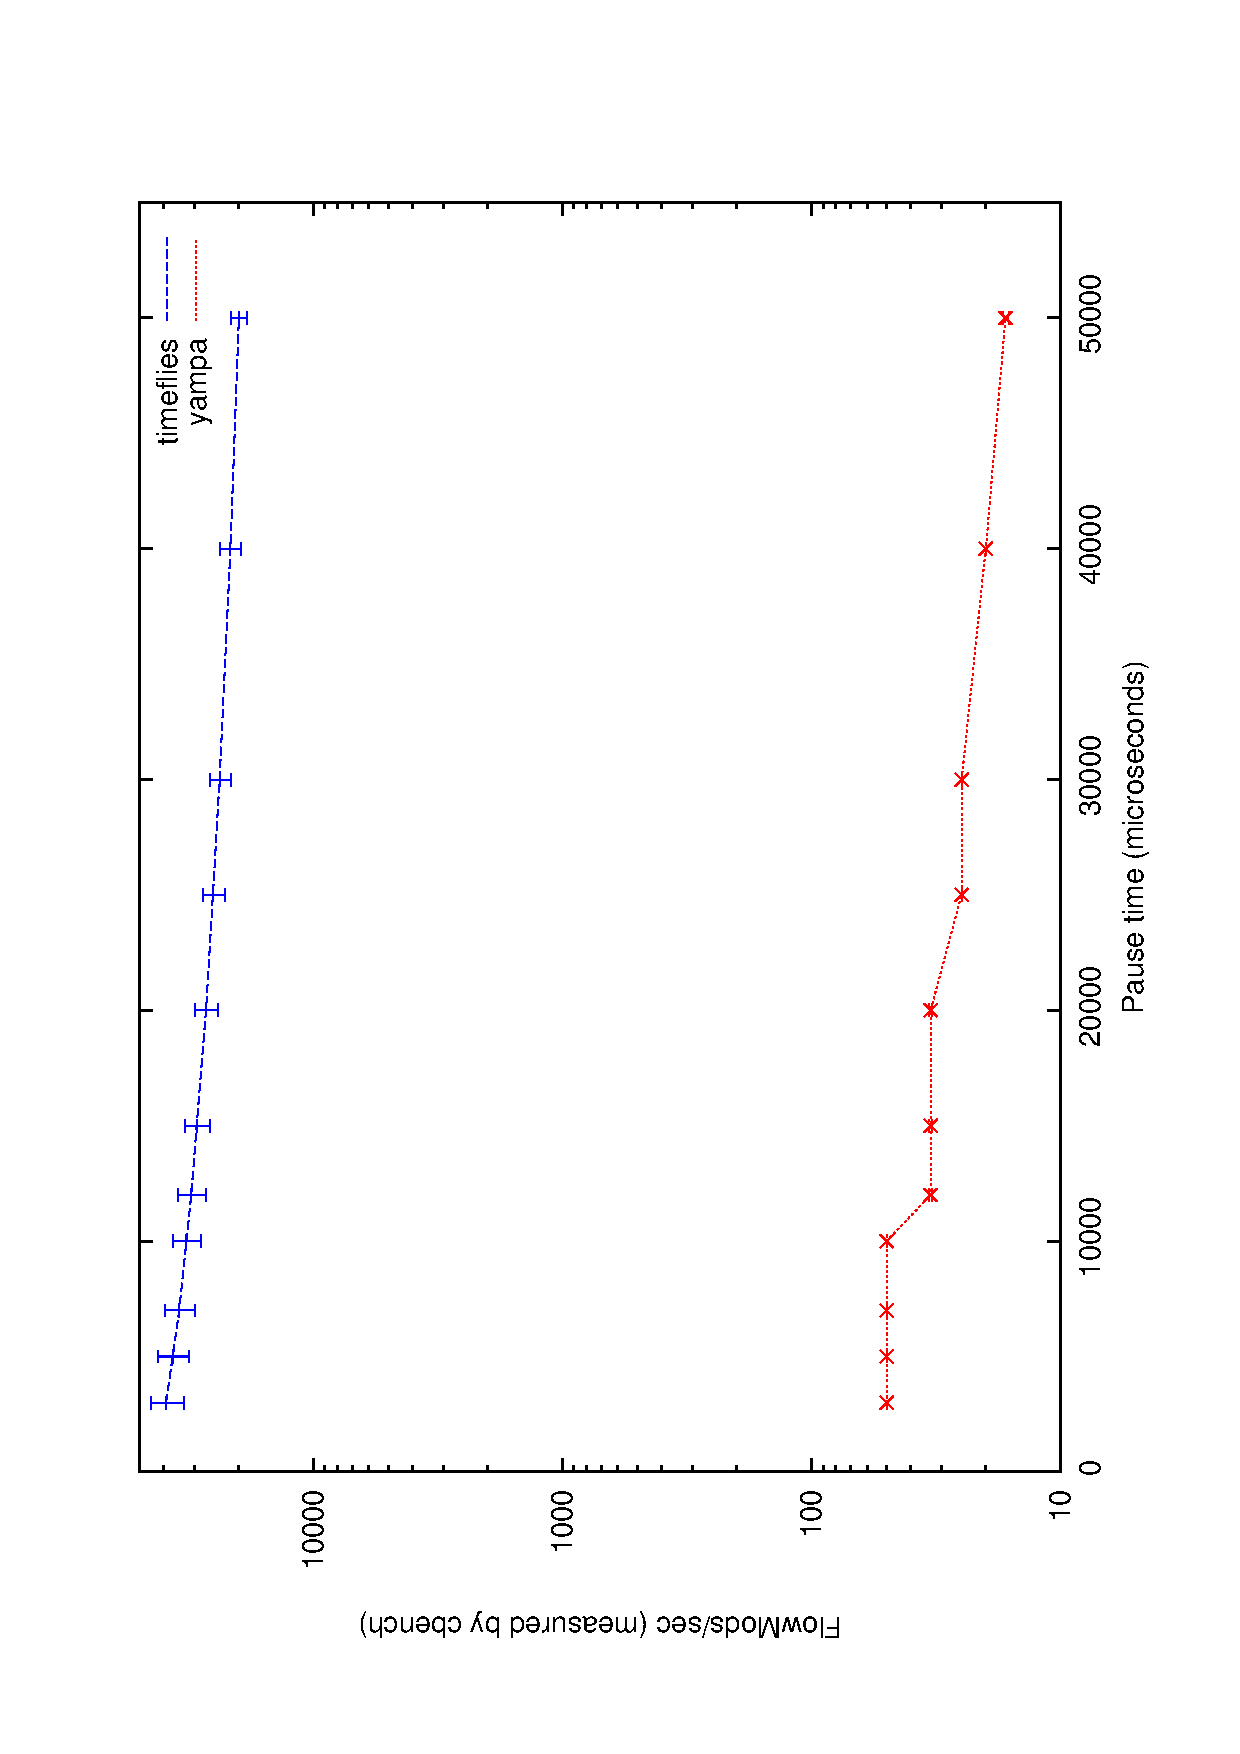
\includegraphics{graph}
\hrule
\caption{Comparison of timeflies vs. Yampa implementing an OpenFlow learning switch controller.}
\label{fig:timeflies-yampa-comparison}
\end{figure}

There is some correlation between the sampling rate and the response rate
for TimeFlies, which is due to the continued wrapping of a replacement signal
function by {\tt switch} until the next time step (see Section~\ref{subsection:Implementation-Signal_Functions-Implementation_of_Signal_Function_Combinators}).
Nevertheless, TimeFlies outperforms Yampa in event response by several orders of magnitude,
even at a very high sampling rate. This is due to two factors. First, TimeFlies can react
to individual events without evaluating the whole signal function. Second, in
the implementation described in Chapter~\ref{chapter:Example_Application}, the
interface of TimeFlies permits us to connect its evaluation directly to GHC's
event manager, while the design of Yampa requires us to use threads and
synchronized communication\footnote{Yampa does include a step-wise evaluation
function, but it still couples event evaluation firmly to time steps, and is not well
documented.}. Even the TimeFlies implementation using polling IO outperforms the
Yampa version, due to the ability to evaluate multiple events per time step.


\chapter{Conclusions and Further Work}
\label{chapter:Conclusions_and_Further_Work}
I have presented TimeFlies, a push-based signal-function FRP system. I have
demonstrated that TimeFlies does realize the theoretical benefits of a
push-based signal-function system.

The TimeFlies system is a full-fledged and documented FRP library which may
be extended with utility functions and further optimized. Its performance in
responding to events is demonstrated to be superior to that of the predominant
pull-based signal-function FRP library.

Further, the model of events used by TimeFlies subverts problematic semantic
questions about the evaluation of events in a system. By using the N-Ary FRP
type model and separating the evaluation of events from the time steps used
for signals, TimeFlies fully supports non-deterministic merging of events,
and provides a semantic guarantee that events are not ''lost'' during evaluation.

The TimeFlies system would benefit from attentive microbenchmarking and performance
tuning, as well as optimizations to avoid evaluating irrelevant parts of the network
during the the evaluation of time steps. A formal semantic justification for the
formulation of event evaluation (which would require a full formal semantics of FRP)
would enable a far more robust correctness argument, as well as providing a basis for
semantic extensions to signal-function FRP.

FRP is not yet mature, and has not been the subject of focused application development.
Thus, there is a dearth of design patterns for FRP applications. Such design patterns
would yield necessary feedback as to which generalizations and restrictions of FRP would
be appropriate and useful, and clarify the necessity of various utility combinators to
be included in the standard libraries of FRP systems.

In order to improve the performance of FRP yet further, it may be productive to attempt
to introduce parallel evaluation into FRP, taking advantage of the functional purity in
the implementation of the signal function combinators. This may involve, for instance,
evaluating several time-steps at once in a data-parallel manner,task parallelism
between different branches of a signal function, or speculative evaluation of switch
combinators.

Many classes of reactive application would benefit from a ``dynamic collections'' combinator
similar to {\tt pSwitch} in Yampa. Such a combinator allows a collection of signal functions
to be evaluated as one signal function, with addition or removal of signal functions instead
of the total replacement given by the {\tt switch} combinator. This is useful, for instance,
when simulating objects for games or computer models, as the behavior of each object can be
modeled as a signal function, and these signal functions can be added to and removed from the
collection.

The TimeFlies system provides a principled and performant system for future experimentation
on FRP, as well as implementation of FRP applications.



%%%%%%%%%%%%%%%%%%%%%%%%%%%%%%%%%%%%%%%%%%%%%%%%%%%%%%%%%%%%%%%%%%%%%%
% Appendix/Appendices                                                %
%%%%%%%%%%%%%%%%%%%%%%%%%%%%%%%%%%%%%%%%%%%%%%%%%%%%%%%%%%%%%%%%%%%%%%
%
% If you have only one appendix, use the command \appendix instead
% of \appendices.
%
\appendix
\index{Appendices@\emph{Appendices}}%

\chapter{Haskell Concepts}
\label{chapter:Haskell_Concepts}

One of the primary attractions of the Haskell language, and the reason for its
use throughout this work, is its advanced yet practical and usable type system.
This type system enables the use of compositional software design that would
be rendered infeasible without a type system to both inform and verify
composition and implementation. This appendix gives an overview of Haskell
concepts, design patterns, and idioms which are used in this thesis.

\section{Datatypes and Pattern Matching}
\label{section:Haskell_Concepts-Datatypes_and_Pattern_Matching}

In Haskell, new type constructors are introduced by defining Algebraic Datatypes.
An ADT declaration can take one of two forms. The first is a {\tt data}
declaration, e.g.:

\begin{code}
data Bool = True | False
data Maybe a = Just a | Nothing
\end{code}

In this form the identifier(s) preceding the {\tt =} character are a type
constructor followed by zero or more type variables. Following the {\tt =} 
character, and separated by {\tt |} characters, are data constructors. Each data
constructor is an identifier followed by zero or more types, which are the types
of its arguments. Data constructors can be used in expressions to construct a
value of this newly-declared type constructor, and in pattern matching to
``take apart'' the value and observe its components (the arguments to the data
constructor.

The second form is the {\tt newtype} declaration. This form is more restricted.
It is limited to one data constructor with exactly one argument. It introduces
a new type without introducing a new runtime restriction, though the Haskell
code must still use the data constructor in pattern matches and expressions
to explicitly coerce between the new type and the type of its data constructor's
parameter. This behavior is most often used to hide implementation types without
introducing the runtime overhead of value construction and pattern-matching, as
these are erased for constructors declared using {\tt newtype} once type-checking
is complete.

Once a type constructor has been introduced, it can be used in a type, with
its arguments replaced by any valid Haskell type. For instance:

\begin{code}
not      :: Bool -> Bool
cbool    :: Bool -> Int
maybeInt :: Int -> Maybe Int -> Int
isJust   :: Maybe a -> Bool
mapMaybe :: (a -> b) -> Maybe a -> Maybe b
\end{code}

Its data constructors can be used in the patterns of functions, and in their
expressions. For instance:

\begin{code}
not :: Bool -> Bool
not True  = False
not False = True

isJust :: Maybe a -> Bool
isJust (Just _) = True
isJust Nothing  = False

mapMaybe :: (a -> b) -> Maybe a -> Maybe b
mapMaybe f (Just x) = Just (f x)
mapMaybe _ Nothing  = Nothing
\end{code}

\subsection{Generalized Algebraic Datatypes}
\label{subsection:Haskell_Concepts-Datatypes_and_Pattern_Matching-Generalized_Algebraic_Datatypes}

GADTs~\cite{Cheney2003,Xi2003} permit us to specify what types fill in the type
parameters for specific constructors. For instance, if we wish to build a tiny
expression language, we can use a standard ADT:

\begin{code}
data Exp a = Const a 
           | Plus (Exp a) (Exp a)
           | LessThan (Exp a) (Exp a)
           | If (Exp a) (Exp a) (Exp a)
\end{code}

Let us assume for the moment that Haskell exports functions\footnote{The types
for addition and comparison actually involve a typeclass constraint, but the
point is that the functions' types are not parametric.}:

\begin{code}
(+)  :: Int -> Int -> Int
(<)  :: Int -> Int -> Bool
\end{code}

An attempt to write an evaluation function for our expression type is:

\begin{code}
eval :: Exp a -> a
eval (Const x)  = x
eval (Plus x y) = eval x + eval y
eval (LessThan x y) = eval x < eval y
eval (If p c a) = if (eval p)
                  then eval c
                  else eval a
\end{code}

But this function will not typecheck. In the {\tt Plus} case, we cannot
assume that the argument to the type constructor {\tt Exp} typing {\tt x} or {\tt y}
is {\tt Int}, and similarly for the {\tt LessThan} case. Again in the {\tt If}
case, we cannot assume that the predicate is of type {\tt Exp Bool}, and if we
could, that would force our results to be of type {\tt Exp Bool} as well.

Let's try a slightly modified ADT:

\begin{code}
data Exp a = Const a
           | Plus (Exp Int) (Exp Int)
           | LessThan (Exp Int) (Exp Int)
           | IfThenElse (Exp Bool) (Exp a) (Exp a)
\end{code}

Here the motivation for a type parameter to our type constructor becomes clear.
We can introduce both {\tt Bool} and {\tt Int} constants (as well as others, but
we cannot do anything with them unless we extend the language). Further, we
can constrain the types of the input expressions to each of our constructors to
be of the appropriate type.

The code for our our evaluator is the same. But now note that the in the
{\tt Plus} and {\tt LessThan} cases, even though the input types are compatible
with the functions used, the output type expected from our function is not.
{\tt Plus x y} has type {\tt Exp a} in the pattern match, so our output is
expected to be of type {\tt a} for any {\tt a} argument to type of an 
input {\tt Exp}.

Here is our expression type as a GADT:
\begin{code}
data Exp a where
  Const    :: a                               -> Exp a
  Plus     :: Exp Int  -> Exp Int             -> Exp Int
  LessThan :: Exp Int  -> Exp Int             -> Exp Bool
  If       :: Exp Bool -> Exp a   -> Exp a    -> Exp a
\end{code}

Now our evaluation function can typecheck. Each constructor is able to constrain
the type parameter for output, not just its arguments. So when pattern matching
on the {\tt Plus} case, we know that each of our inputs will be of type
{\tt Exp Int}, and that the type of the expression we are pattern matching has
type {\tt Exp Int}, so the output from our function can be constrained to type
{\tt Int}, similarly for {\tt LessThan}. The type argument to {\tt Exp} in the
type of the {\tt If} is constrainted to be the same as that as the argument
to the types of the consequent and alternate to the conditional. This permits
our {\tt If} statement to be parametric while still allowing our evaluation to
typecheck.

This capacity to constrain the output types of data constructors, and thus, to
constrain the types of expressions in the scope of pattern matches of these data
constructors, is called {\em type refinement}. We will make use of this ability
to parameterize concrete datatypes over abstract type structures, rather than to
permit typechecking in specific cases, but the principle is the same.

\section{Typeclasses}
\label{section:Haskell_Concepts-Typeclasses}

Typeclasses in Haskell provide a means to implement functions that are openly
polymorphic while not being parametric. A typeclass is declared as follows:

\begin{code}
class Show t where
  show :: t -> String
\end{code}

A typeclass has an identifier and a single type parameter. This type parameter
is used in the type of one or more functions which are members of the class.

The class can then be instantiated:

\begin{code}
instance Show Bool where
  show True  = "True"
  show False = "False"

instance (Show a) => Show (Maybe a) where
  show (Just x) = "Just " ++ show x
  show Nothing  = Nothing
\end{code}

Functions can now be written polymorphically over the types instantiating the
typeclass, by including the typeclass as a constraint:

\begin{code}
repL :: (Show t) => t -> Int
repL x = length (show x)
\end{code}

Typeclasses are used in Haskell to provide common interfaces or functionality
across types. The {\tt Show} class used as an example is exported, along with
instances for most of the basic Haskell types, from Haskell's Prelude (the
standard module imported into every Haskell module). 

\section{Monads and Monad Transformers}
\label{section:Haskell_Concepts-Monads_and_Monad_Transformers}

One of the primary concepts employed in Haskell programs is that of the
monad~\cite{PeytonJones1993,PeytonJones2001}. The concept of the monad is
borrowed from category theory, but it is quite simple when understood within
Haskell. A monad is a type constructor with a single parameter, and two
associated functions. In Haskell's {\tt Monad} typeclass, these functions are
denoted {\tt return} and {tt (>>=)}.

\begin{code}
class Monad m where
  return :: a -> m a
  (>>=)  :: m a -> (a -> m b) -> m b
\end{code}

A monad must obey the following axioms:
\begin{itemize}
\item Left identity: {\tt return x >>= f = f x}
\item Right identity: {\tt m >>= return = m}
\item Associativity: {\tt (a >>= b) >>= c) = (a >>= (\\x -> b x >>= c))}
\end{itemize}

Several standard Haskell type constructor are monads in interesting ways, but
the most well-known is Haskell's {\tt IO} type constructor. This is the basis of
Haskell's input/output system. The entry point to a Haskell program is the
{\tt main} function, of type {\tt IO ()}. This function can be constructed by
using the monadic functions to sequence an arbitrary number of other functions
whose output type is {\tt IO a}. Since the sequencing operator takes an
arbitrary function, this allows the full power of Haskell functions, including
first-class and higher-order functions, to be employed in defining a program's
input and output. A convenience function is commonly used when the result is not
necessary as part of the sequencing:

\begin{code}
(>>) :: Monad m => m a -> m b -> m b
(>>) m1 m2 = m1 >>= (const m2)

\subsection{Do-notation}
\label{subsection:Haskell_Concepts-Monads_and_Monad_Transformers-Do_notation}

Because monads are such a pervasive concept in Haskell, the language includes
special syntax for writing monadic expressions. Do-notation is expression syntax
which begins with the keyword {\tt do} and is followed by lines of two forms:

\begin{code}
do
  x <- m1
  m2
\end{code}

The first form is a binding expression: it binds the variable {\tt x} to the
output of the monadic value {\tt m2}. The second form simply sequences the monad
value {\tt m2} into the monadic value being built. Do-notation has a syntax-driven
translation to desugared Haskell expression:

\begin{code}
desugar {
do x <- m1
   ...} = 
m1 >>= \x -> desugar {do ...}

desugar {
do m1
   ...} =
m1 >> desugar {do ...}
\end{code}

\subsection{Monad Transformers}
\label{subsection:Haskell_Concepts-Monads_and_Monad_Transformers-Monad_Transformers}
A monad transformer is a type constructor with two parameters. The first
parameter parameterizes over a one-parameter type constructor, rather than a
type. The second is the monadic type parameter. A type constructor {T} is a monad
transformer if it has the following instance of the Monad typeclass:

\begin{code}
instance Monad m => Monad T m
\end{code}

and is also an instance of the class

\begin{code}
class MonadTrans t where
  lift :: (Monad m) => m a -> t m a
\end{code}

The axioms for the lift function are:
\begin{itemize}
\item {\tt lift . return = return}
\item {\tt lift (m >>= f) = lift m >>= (lift . f)}
\end{itemize}

Restated, {\tt lift} does not modify return and distributes over monadic
sequencing.

As an example of a monad transformer, we can consider the {\tt StateT} type,
which is employed in the implementation of this thesis.

The type is declared:
\begin{code}
newtype StateT s m a = S { runStateT :: s -> m (s, a) }
\end{code}

Its monad instance, for any {\tt s}, is

\begin{code}
instance Monad m => Monad (StateT s m) where
  return x  = S (\s -> return (x, s))
  (>>=) (S f) mf = S (\s -> f s >>= (\ (x, s') -> let (S f') = mf x in f' s ))
\end{code}

The return and sequencing functions carry the state through the underlying monad.

The {\tt MonadTrans} instance is:
\begin{code}
instance MonadTrans (StateT s) where
  lift m = S (\s -> m >>= (\x -> return (x, s))
\end{code}

Finally, there are two functions provided to access and set the state:

\begin{code}
put :: s -> StateT s m ()
put = S (\_ -> return ((), s'))

get :: StateT s m s
get = S (\s -> return (s, s))
\end{code}

If we use {\tt StateT} as a wrapper around the IO monad, we might employ it as
a way to generate a unique line number for each "putStrLn" we call.

\begin{code}
putStrLnN :: String -> StateT Int IO ()
putStrLnN s = do i <- get
                 put (i + 1)
                 lift (putStrLn (show i ++ " " ++ s))

main = runStateT mainSt 1
  where mainSt = do g <- lift getLine
                    putStrLnN g
                    mainSt
\end{code}

\chapter{Glossary of Type Terminology}
\label{chapter:Haskell_Concepts-Glossary_of_Type_Terminology}
\begin{description}
\item[ADT] See {\em Algebraic Datatype}.

\item[Algebraic Datatype] An Algebraic Datatype or ADT is a type whose terms
are {\em data constructors}. An ADT is defined by naming a
{\em type constructor} and its parameters (zero or more)
(as {\em type variables}), together with one or more data constructors and the
types of their members. Each data constructor takes a fixed number
(zero or more) data members, whose types are given following the constructor
name. These types are defined in terms of the type variables named as parameters
of the type constructor and any type constructors (including the type
constructor associated with the ADT) in scope in the module.

\item[Data Constructor] A Data Constructor is a component of an
Algebraic~Datatype which, when applied to values of the appropriate type, 
creates a value typed with the ADT. Data constructors are the primary element
which may be pattern matched in languages such as Haskell.

\item[GADT] See {\em Generalized Algebraic Datatype}.

\item[Generalized Algebraic Datatype] Similar to an {\em Algebraic Datatype},
but {\em type variables} in the {\em type constructor} declaration serve merely
to denote the number of type parameters (and thus may be replaced by a
{\em kind signature}) and types are given for each {\em data constructor}. These
types must have the type constructor as their top-level term, but may fill in
the parameters of the type constructor with arbitrary types. Variables which
appear in the data member types but on in the data constructor type are
{\em existentially quantified}, and types appearing in the data constructor
type but not the data member types may be instantiated arbitrarily.

\item[Kind] A ``type of types.'' Kinds are used to verify that types are
consistent during typechecking. The kind of types which contain values is
{\tt *}, and the kind of single-parameter type constructors which take a
type is {\tt * -> *}. Other kinds may also be introduced. For instance,
signal vectors should be their own separate kind, but the Haskell type mechanism
was not mature enough to support this at the time of this writing..

\item[Kind Signature] A means of specifying the number and kind of types which
may instantiate type variables. Type variables in Haskell are not restricted to
types, but may be instantiated by type constructors as well. The kind of a
variable restricts what it may be instantiated with. A kind signature gives
kinds to a type constructor, and thus to its parameters. Specifying the kind
of a type constructor perfectly constrains the number of parameters.

\item[Type Constructor] A type constructor is a type level term which, when
applied to the proper number of types, produces a type. Type constructors,
together with {\em type variables}, form the basis of polymorphism in Haskell
and similar languages.

\item[Type Variable] A type variable is a type-level term which may be 
instantiated (by the typechecker via inference, or by the user via annotation)
with any type at the point where the value so typed is used. 
Together with {\em type constructors}, type variables form the basis of
polymorphism in Haskell and similar languages.
\end{description}


%\include{chapter-appendix2}

%\include{chapter-appendix3}


%%%%%%%%%%%%%%%%%%%%%%%%%%%%%%%%%%%%%%%%%%%%%%%%%%%%%%%%%%%%%%%%%%%%%%
% Generate the bibliography.                         %
%%%%%%%%%%%%%%%%%%%%%%%%%%%%%%%%%%%%%%%%%%%%%%%%%%%%%%%%%%%%%%%%%%%%%%
%                                    %
% NOTE: For master's theses and reports, NOTHING is permitted to     %
%   come between the bibliography and the vita. The command      %
%   to generate the index (if used) MUST be moved to before      %
%   this section.                            %
%                                    %
%
%\nocite{*}      % This command causes all items in the           %
                % bibliographic database to be added to          %
                % the bibliography, even if they are not         %
                % explicitly cited in the text.              %
        %                            %
  % Here the bibliography           %
        % is inserted.                %

\index{Bibliography@\emph{Bibliography}}%
\bibliographystyle{plain}
\bibliography{thesis}
%%%%%%%%%%%%%%%%%%%%%%%%%%%%%%%%%%%%%%%%%%%%%%%%%%%%%%%%%%%%%%%%%%%%%%


%%%%%%%%%%%%%%%%%%%%%%%%%%%%%%%%%%%%%%%%%%%%%%%%%%%%%%%%%%%%%%%%%%%%%%
% Generate the index.                            %
%%%%%%%%%%%%%%%%%%%%%%%%%%%%%%%%%%%%%%%%%%%%%%%%%%%%%%%%%%%%%%%%%%%%%%
%                                    %
% NOTE: For master's theses and reports, NOTHING is permitted to     %
%   come between the bibliography and the vita. This section     %
%   to generate the index (if used) MUST be moved to before      %
%   the bibliography section.                    %
%                                    %
%\printindex%    % Include the index here. Comment out this line      %
%       % with a percent sign if you do not want an index.   %
%%%%%%%%%%%%%%%%%%%%%%%%%%%%%%%%%%%%%%%%%%%%%%%%%%%%%%%%%%%%%%%%%%%%%%


%%%%%%%%%%%%%%%%%%%%%%%%%%%%%%%%%%%%%%%%%%%%%%%%%%%%%%%%%%%%%%%%%%%%%%
% Vita page.                                 %
%%%%%%%%%%%%%%%%%%%%%%%%%%%%%%%%%%%%%%%%%%%%%%%%%%%%%%%%%%%%%%%%%%%%%%
\begin{vita}
Edward Amsden was born in Dayton, Ohio in the year 1990, to Andrew and
Vivian Amsden. He is pursuing concurrent B.S. and M.S. degrees at the Rochester
Institute of Technology. Once his M.S. is completed, he plans to begin his
Ph.~D. at Indiana University. His research interests include functional
programming languages, concurrency and parallelism, computer graphics, and
computer audio. 
\end{vita}
\end{document}
